\section{Hardware}
\label{sec:Hardware}



\begin{itemize}
    \item HX711
    \item Arduino UNO (ATMEGA328p)
    \item TMC2209 Driver
    \item Schaltplan
    \item Wägezelle
    \item Steppermotor ACT 24HS5430D8L2
    full step $1,8 \pm 5$ per step;
    3 A/phase;
    2,4 V;
    150 N.cm Haltemoment;
    350 $g \cdot cm^2$ Drehmoment;
    \item Netzteil
    \item Stepdownconverter
\end{itemize}


% \item  Bitte keine Copy+Paste Texte vom Hersteller in Text oder Präsentation
% Kurz und knackig, was kann der Sensor
% Was ist das physikalische Messprinzip
% Sensor/Aktor Kalibrierung
%     Wie haben Sie gewährleistet, dass der Sensor richtig misst?
%     Was ist ihr Normativ?
%     Wie hoch ist die Standardabweichung des Sensors im Ruhezustand mit/ohne System?


\begin{figure}[H]
    \centering
    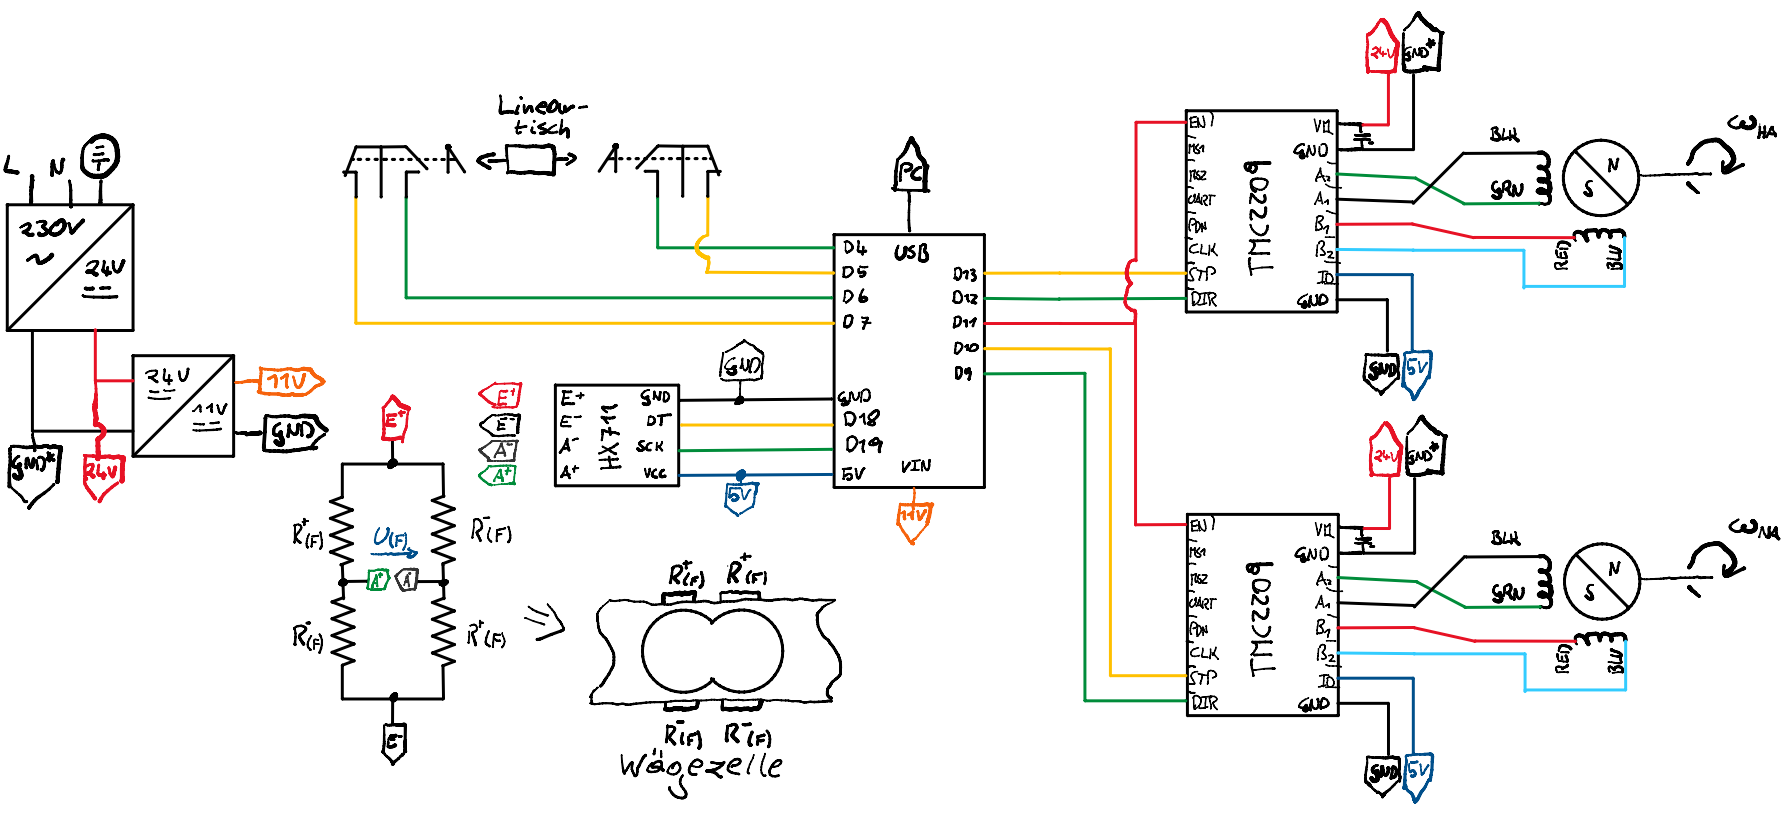
\includegraphics[width=1\textwidth]{./schaltplan.png}
    \caption{Schaltplan}
    \label{fig:schaltplan}
\end{figure}





